\section{Families of Continuous Distributions}

As in the discrete case, varieties of phenomena can be described by relatively few families of continuous distributions. Here, we shall discuss \textit{\textbf{Uniform, Exponential, Gamma}}, and \textit{\textbf{Normal}} families, adding Student's $t$, Pearson's $\chi^2$, and Fisher's $F$ distributions in later chapters.

\subsection{Uniform Distribution}

\textit{\textbf{Uniform distribution}} plays a unique role in stochastic modeling. A random variable with any thinkable distribution can be generated from a Uniform random variable. Many computer languages and software are equipped with a random number generator that produces Uniform random variables. Users can convert them into variables with desired distributions and use for computer simulation of various events and processes.

Also, Uniform distribution is used in any situation when a value is picked ``at random'' from a given interval; that is, without any preference to lower, higher, or medium values. For example, locations of errors in a program, birthdays throughout a year, and many continuous random variables modulo 1, modulo 0.1, 0.01, etc., are uniformly distributed over their corresponding intervals.

To give equal preference to all values, the Uniform distribution has a \textit{constant density} (Figure 3). On the interval $(a, b)$, its density equals
\begin{equation*}
    f(x) = \frac{1}{b - a},\ \ \ \ a < x < b
\end{equation*}
because the rectangular area below the density graph must equal 1.

\begin{figure}[ht]
    \centering
    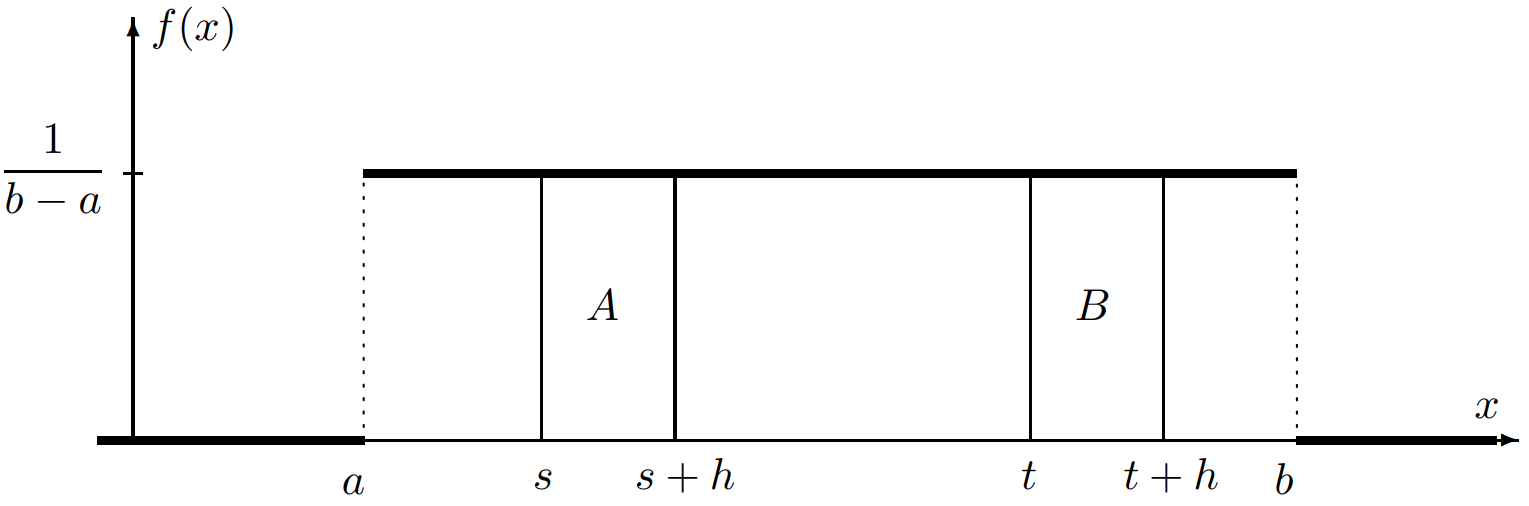
\includegraphics[width=.5\textwidth]{img/Fig4.4.png}
    \caption{\textit{The Uniform density and the Uniform property.}}
\end{figure}

For the same reason, $| b - a |$ has to be a finite number. There does not exist a Uniform distribution on the entire real line. In other words, if you are asked to choose a random number from $(-\infty, +\infty)$, you cannot do it uniformly.

\subsubsection{The Uniform Property}

For any $h > 0$ and $t \in \left[ a, b - h \right]$, the probability
\begin{equation*}
    \prob{t < X < t + h} = \int_t^{t+h} \frac{1}{b - a} dx = \frac{h}{b - a}
\end{equation*}
is \textit{independent} of $t$. This is the \textit{\textbf{Uniform property}}: the probability is only determined by the length of the interval, but not by its location.

\begin{example}{}
In Figure 3, rectangles $A$ and $B$ have the same area, showing that
\begin{equation*}
    \prob{s < X < s + h} = \prob{t < X < t + h}
\end{equation*}
\end{example}

\subsubsection{Standard Uniform Distribution}

The Uniform distribution with $a = 0$ and $b = 1$ is called \textit{Standard Uniform distribution}. The Standard Uniform density is $f(x) = 1$ for $0 < x < 1$. Most random number generators return a Standard Uniform random variable.

All the Uniform distributions are related in the following way. If $X$ is a Uniform$(a, b)$ random variable (\textit{not standard uniform random variable}), then
\begin{equation*}
    Y = \frac{X - a}{b - a}
\end{equation*}
is Standard Uniform \textit{(If X is not inside (0,1), ``X-a'' slides X to the (0,1))}. Likewise, if $Y$ is Standard Uniform, then
\begin{equation*}
    X = a + (b-a)Y
\end{equation*}
is Uniform$(a, b)$. Check that $X \in (a, b)$ if and only if $Y \in (0, 1)$.

A number of other families of distributions have a ``standard'' member. Typically, a simple transformation converts a standard random variable into a non-standard one, and vice versa.

\subsubsection{Expectation and Variance}

For a Standard Uniform variable $Y$,
\begin{equation*}
    \expc{Y} = \int y f(y)dy = \int_0^1 ydy = \frac{1}{2}
\end{equation*}
and
\begin{equation*}
    \var{Y} = \expc{Y^2} - \mathbf{E}^2(Y) = \int_0^1 y^2dy - \left( \frac{1}{2} \right)^2 = \frac{1}{3} - \frac{1}{4} = \frac{1}{12}
\end{equation*}

Now, consider the general case (\textit{Case of not being the standard uniform}). Let $X = a+(b-a)Y$ which has a Uniform$(a, b)$ distribution. By the properties of expectations and variances,
\begin{equation*}
    \expc{X} = \expc{a + (b - a)Y} = a + (b - a)\expc{Y} = a + \frac{b-a}{2} = \frac{a+b}{2}
\end{equation*}
and
\begin{equation*}
    \var{X} =\var{a + (b - a)Y} = (b - a)^2 \var{Y} = \frac{(b - a)^2}{12}
\end{equation*}
The expectation is precisely the middle of the interval $\left[ a, b \right]$. Giving no preference to left or right sides, this agrees with the Uniform property and with the physical meaning of $\expc{X}$ as a center of gravity.

\subsubsection{Uniform Distribution Functions and Variables}
\begin{formula}{Uniform Distribution}
\begin{center}
$\begin{aligned}
    (a, b) &= \text{range of values}\\
    f(x) &= \frac{1}{b - a},\ \ \ \ a < x < b\\
    \expc{X} &= \frac{a+b}{2}\\
    \var{X} &= \frac{(b - a)^2}{12}
\end{aligned}$
\end{center}
\end{formula}

\subsection{Exponential Distribution}

\textbf{\textit{Exponential distribution}} is often used to model \textit{time}: waiting time, interarrival time, hardware lifetime, failure time, time between telephone calls, etc. As we shall see below, in a sequence of rare events, \textit{when the number of events is Poisson, the time between events is Exponential.}

Exponential distribution has density
\begin{equation}
    f(x) = \lambda e^{-\lambda x} \textnormal{ for } x > 0
\end{equation}
With this density, we compute the Exponential cdf, mean, and variance as
\begin{align}
    \prob{X \leq x} = F(x) &= \int_0^x f(t)dt = \int_0^x \lambda e^{-\lambda t} dt = 1 - e^{-\lambda x} \textnormal{    ($x > 0)$}\\
    \expc{X} &= \int tf(t)dt = \int_0^{\infty} t \lambda e^{-\lambda t} = \frac{1}{\lambda} \textnormal{    (integral by parts)}\\
    \var{X} &= \int t^2 f(t)dt - \mathbf{E}^2(X) \nonumber \\
    &= \int_0^{\infty} t^2 \lambda e^{-\lambda t} dt - \left( \frac{1}{\lambda} \right)^2 \textnormal{    (by parts twice)} \nonumber \\
    &= \frac{2}{\lambda^2} - \frac{1}{\lambda^2} = \frac{1}{\lambda^2}
\end{align}
The quantity $\lambda$ is a parameter of Exponential distribution, and its meaning is clear from $\expc{X} = 1/\lambda$. If $X$ is time, measured in minutes, then $\lambda$ is a frequency, measured in min$^{-1}$. For example, if arrivals occur every half a minute, on the average, then $\expc{X} = 0.5$ and $\lambda = 2$, saying that they occur with a frequency (arrival rate) of 2 arrivals per minute. This $\lambda$ has the same meaning as the parameter of Poisson distribution.
\begin{formula}{Important Note}
    \begin{center}
    $\prob{X > x} = 1 - \prob{X \leq x} = 1 - (1 - e^{-\lambda x}) = e^{-\lambda x}$
    \end{center}
    In here $X$ is ``\textit{time between two events}'' and $x$ is ``\textit{particular time}''. So, if this particular time, $x$, is greater than or equal to time between two events, $X$, the eq. 2 is used. Otherwise, the equation inside this box is used.

    \quad ``\textbf{\textit{Exponential distribution}} is a continuous version of \textbf{\textit{Geometric distribution}}. In the \textit{Geometric distribution}, we analyze the how many trials are required before the first success, whereas, in the \textit{Exponential distribution}, we analyze the time until the first success.''
\end{formula}

\subsubsection{Times between rare events are Exponential}

What makes Exponential distribution a good model for interarrival times? Apparently, this is not only experimental, but also a mathematical fact.

As in Chapter 3, consider the sequence of rare events, where the number of occurrences during time $t$ has Poisson distribution with a parameter proportional to $t$. 

Event ``the time $T$ until the next event is greater than $t$'' can be rephrased as ``zero events occur by the time $t$'', and further, as ``$X = 0$'', where $X$ is the number of events during the time interval $\left[ 0, t \right]$ (\textit{It is related with the note in previous page}). This $X$ has Poisson distribution with parameter $\lambda t$. It equals 0 with probability
\begin{equation*}
    P_X(0) = e^{-\lambda t} \frac{(\lambda t)^2}{0!} = e^{-\lambda t}
\end{equation*}
Then we can compute the cdf of $T$ as
\begin{equation}
    F_T(t) = 1 - \prob{T > t} = 1 - \prob{X = 0} = 1 - e^{-\lambda t}
\end{equation}
and here we recognize the Exponential cdf. Therefore, the time until the next arrival has Exponential distribution.

\begin{example}{}
Jobs are sent to a printer at an average rate of 3 jobs per hour.

(a) What is the expected time between jobs?
(b) What is the probability that the next job is sent within 5 minutes?

\textbf{Solution:}
Job arrivals represent rare events, thus the time $T$ between them is Exponential with the given parameter $\lambda = 3$ hrs$^{-1}$ (jobs per hour).

(a) $\expc{T} = 1/\lambda = 1/3$ hours or 20 minutes between jobs.

(b) Convert to the same measurement unit: 5 min = (1/12) hrs. Then,
\begin{equation*}
    \prob{T < 1/12 \textnormal{ hrs}} = F(1/12) = 1 - e^{-\lambda (1/12)} = 1 - e^{1/4} = 0.2212
\end{equation*}
\end{example}

\subsubsection{Memoryless Property}

It is said that ``Exponential variables lose memory''. What does it mean?

Suppose that an Exponential variable $T$ represents waiting time. Memoryless property means that the fact of having waited for $t$ minutes gets ``\textit{forgotten}'', and it \textit{does not affect the future waiting time}. Regardless of the event $T > t$, when the total waiting time exceeds $t$, the remaining waiting time still has Exponential distribution with the same parameter. Mathematically,
\begin{equation}
    \prob{T > t + x\ |\ T > t} = \prob{T > x}\ \ \ \ \textnormal{ for } t, x > 0
\end{equation}
In this formula, $t$ is the already elapsed portion of waiting time, and $x$ is the additional, remaining time.
\begin{proof}
    $\prob{T > x} = e^{-\lambda x}$. Also, by the formula for conditional probability,
    \begin{equation*}
        \prob{T > t + x\ |\ T > t} = \frac{\prob{T > t + x \cap T > t}}{\prob{T > t}} = \frac{\prob{T > t + x}}{\prob{T > t}} = \frac{e^{-\lambda (t+x)}}{e^{-\lambda t}} = e^{-\lambda x}
    \end{equation*}
\end{proof}
This property is unique for Exponential distribution. No other continuous variable $X \in (0, \infty)$ is memoryless. Among discrete variables, such a property belongs to Geometric distribution.

\subsubsection{Exponential Distribution Functions and Variables}

\begin{formula}{Exponential Distribution}
\begin{center}
    $\begin{aligned}
        \lambda &= \textnormal{frequency parameter, the number of events
        per time unit}\\
        f(x) &= \lambda e^{-\lambda x},\ \ \ \ x > 0\\
        \expc{X} &= \frac{1}{\lambda}\\
        \var{X} &= \frac{1}{\lambda^2}
    \end{aligned}$
\end{center}
\end{formula}

\subsection{Gamma Distributinon}

When a certain procedure consists of $\alpha$ independent steps, and each step takes Exponential($\lambda$) amount of time, then the total time has \textit{\textbf{Gamma distribution}} with parameters $\alpha$ and $\lambda$.

Thus, Gamma distribution can be widely used for the total time of a multistage scheme, for example, \textit{related to downloading or installing a number of files}. In a process of rare events, with Exponential times between any two consecutive events, the time of the $\alpha$-th event has Gamma distribution because it consists of $\alpha$ independent Exponential times.

\begin{example}{: Internet Promotions}
    Users visit a certain internet site at the average rate of 12 hits per minute. Every sixth visitor receives some promotion that comes in a form of a flashing banner. Then the time between consecutive promotions has Gamma distribution with parameters $\alpha = 6$ and $\lambda = 12$. 
\end{example}

Having two parameters, Gamma distribution family offers a variety of models for positive random variables. Besides the case when \underline{\textit{a Gamma variable represents a sum of independent Exponential variables}}, Gamma distribution is often used for \textit{the amount of money being paid, amount of a commodity being used (gas, electricity, etc.), a loss incurred by some accident}, etc.

Gamma distribution has a density
\begin{equation}
    f(x) = \frac{\lambda^{\alpha}}{\Gamma(\alpha)} x^{\alpha-1}e^{-\lambda x},\ \ \ \ x > 0
\end{equation}

The denominator contains a Gamma function, later. With certain techniques, this density can be mathematically derived for integer $\alpha$ by representing a Gamma variable $X$ as a sum of Exponential variables each having a density (eq. 1).

In fact, $\alpha$ can take \textit{any positive value}, not necessarily integer. With different $\alpha$, the Gamma density takes different shapes (Figure 4.5). For this reason, $\alpha$ is called a \textit{shape parameter}.

\begin{figure}[h!]
    \centering
    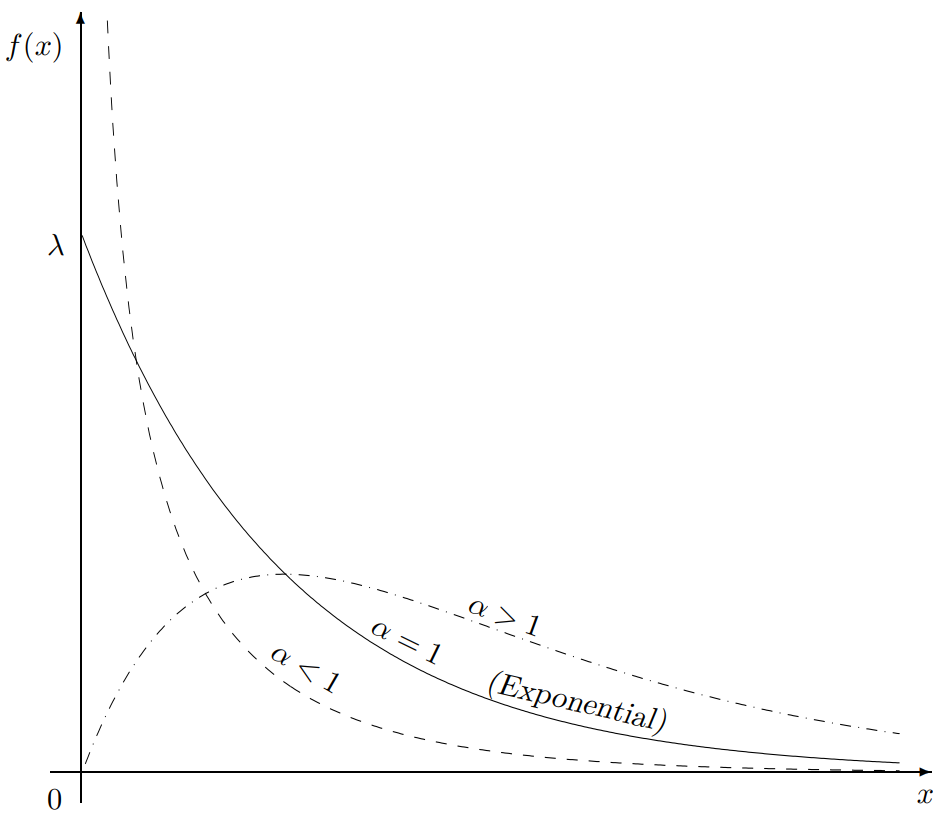
\includegraphics[width=.35\textwidth]{img/Fig4.5.png}
    \caption{\textit{Gamma densities with different shape parameters $\alpha$.}}
\end{figure}

Notice two important special cases of a Gamma distribution. When $\alpha = 1$, the Gamma distribution becomes Exponential. This can be seen comparing (eq. 7) and (eq. 1) for $\alpha = 1$. Another special case with $\lambda = 1/2$ and any $\alpha > 0$ results in a so-called \textit{Chi-square distribution} with ($2\alpha$) degrees of freedom.

\begin{formula}{Special Cases}
    \begin{center}
        $\begin{aligned}
            \textnormal{Gamma}(1, \lambda) &= \textnormal{Exponential}(\lambda)\\
            \textnormal{Gamma}(\alpha, 1/2) &= \textnormal{Chi-square}(2\alpha)\\
        \end{aligned}$
    \end{center}
\end{formula}

\subsubsection{Expectation, Variance, and some useful integration remarks}

Gamma cdf has the form
\begin{equation}
    F(t) = \int_{0}^{t} f(x)dx = \frac{\lambda^{\alpha}}{\Gamma(\alpha)} \int_{0}^{t} x^{\alpha-1} e^{-\lambda x} dx
\end{equation}

This expression, related to a so-called \textit{incomplete Gamma function}, does not simplify, and thus, computing probabilities is not always trivial. Let us offer several computational shortcuts.

First, let us notice that $\begin{aligned}\int_{0}^{\infty} f(x)dx = 1\end{aligned}$ for Gamma and all the other densities. Then, integrating (eq. 7) from $0$ to $\infty$, we obtain that
\begin{equation}
    \int_{0}^{\infty} x^{\alpha-1}e^{-\lambda x} dx = \frac{\Gamma(\alpha)}{\lambda^{\alpha}}\ \ \ \ \textnormal{for any $\alpha > 0$ and $\lambda > 0$}
\end{equation}
Substituting $\alpha + 1$ and $\alpha + 2$ in place of $\alpha$, we get for a Gamma variable $X$
\begin{equation}
    \expc{X} = \int_{}^{} xf(x)dx = \frac{\lambda^{\alpha}}{\Gamma(\alpha)} \int_{0}^{\infty} x^{\alpha} e^{-\lambda x} dx = \frac{\lambda^{\alpha}}{\Gamma(\alpha)} \cdot \frac{\Gamma(\alpha+1)}{\lambda^{\alpha+1}} = \frac{\alpha}{\lambda}
\end{equation}
(using the equality $\Gamma(t + 1) = t \Gamma(t)$ that holds for all t > 0),
\begin{equation*}
    \expc{X^2} = \int_{}^{} x^2f(x)dx = \frac{\lambda^{\alpha}}{\Gamma(\alpha)} \int_{0}^{\infty} x^{\alpha+1} e^{-\lambda x} dx = \frac{\lambda^{\alpha}}{\Gamma(\alpha)} \cdot \frac{\Gamma(\alpha+2)}{\lambda^{\alpha+2}} = \frac{(\alpha + 1) \alpha}{\lambda^2}
\end{equation*}
and therefore,
\begin{equation}
    \var{X} = \expc{X^2} - \expcs{X} = \frac{(\alpha+1)\alpha - \alpha^2}{\lambda^2} = \frac{\alpha}{\lambda^2}
\end{equation}
For $\alpha = 1$, this agrees with (eq. 3) and (eq. 4). Moreover, for any integer $\alpha$, (eq. 10) and (eq. 11) can be obtained directly from (eq. 3) and (eq. 4) by representing a Gamma variable $X$ as a sum of independent Exponential($\lambda$) variables $X_1, ..., X_{\alpha}$,
\begin{align*}
    \expc{X} &= \expc{X_1 + ... + X_{\alpha}} = \expc{X_1} + ... + \expc{X_{\alpha}} = \alpha \left( \frac{1}{\lambda} \right)\\
    \var{X} &= \var{X_1 + ... + X_{\alpha}} = \var{X_1} + ... + \var{X_{\alpha}} = \alpha \left( \frac{1}{\lambda^2} \right)\\
\end{align*}

\subsubsection{Gamma Distribution Functions and Variables}

\begin{formula}{Gamma Distribution: Eq. 12}
\begin{center}
    $\begin{aligned}
        \alpha &= \textnormal{shape parameter}\\
        \lambda &= \textnormal{frequency parameter}\\
        f(x) &= \frac{\lambda^{\alpha}}{\Gamma(\alpha)} x^{\alpha-1} e^{-\lambda x},\ \ \ \ x > 0\\
        \expc{X} &= \frac{\alpha}{\lambda}\\
        \var{X} &= \frac{\alpha}{\lambda^2}
    \end{aligned}$
\end{center}
\end{formula}
\setcounter{equation}{12}

\begin{example_break}{: Total compilation time}
    Compilation of a computer program consists of 3 blocks that are processed sequentially, one after another. Each block takes Exponential time with the mean of 5 minutes, independently of other blocks.\\
    
    (a) Compute the expectation and variance of the total compilation time.
    
    (b) Compute the probability for the entire program to be compiled in less than 12 minutes.\\
    
    \textbf{Solution:} The total time $T$ is a sum of three independent Exponential times, therefore, it has Gamma distribution with $\alpha = 3$. The frequency parameter $\lambda = (1/5)\ min^{-1}$ because the Exponential compilation time of each block has expectation $1/\lambda = 5\ min$. \\

    (a) For a Gamma random variable $T$ with $\alpha = 3$ and $\lambda = 1/5$,
    \begin{align*}
        &\expc{T} = \frac{3}{1/5} = 15\ (min) & \textnormal{and} && \var{T} = \frac{3}{(1/5)^2} = 75\ (min^2)
    \end{align*}

    (b) A direct solution involves two rounds of integration by parts,
    \begin{align}
        \prob{T < 12} &= \int_{0}^{12} f(t)dt = \frac{(1/5)^3}{\Gamma(3)} \int_{0}^{12} t^2 e^{-t/5} dt \nonumber\\
        &= \frac{(1/5)^3}{2!} \left( -5t^2e^{-t/5} \Big|^{t=12}_{t=0} + \int_{0}^{12} 10te^{-t/5}dt \right) \nonumber\\
        &= \frac{(1/125)}{2} \left( -5t^2e^{-t/5} - 50te^{-t/5} \Big|^{t=12}_{t=0} + \int_{0}^{12} 50e^{-t/5}dt \right) \nonumber\\
        &= \frac{1}{250} \left( -5t^2e^{-t/5} - 50te^{-t/5} - 250e^{-t/5}dt \right)\Big|^{t=12}_{t=0} \nonumber\\
        &= 1 - e^{-2.4} - 2.4e^{-2.4} - 2.88 e^{-2.4} = 0.4303
    \end{align}
    A much shorter way is to apply the Gamma-Poisson formula below (example 6).
\end{example_break}

\subsubsection{Gamma-Poisson Formula}

Computation of Gamma probabilities can be significantly simplified by thinking of a Gamma variable as the time between some rare events. In particular, one can avoid lengthy integration by parts, as in Example 5, and use Poisson distribution instead.

Indeed, let $T$ be a Gamma variable with an integer parameter $\alpha$ and some positive $\lambda$. This is a distribution of the time of the $\alpha$-th rare event. Then, the event $\{T > t\}$ means that the
$\alpha$-th rare event occurs after the moment $t$, and therefore, \textit{fewer than $\alpha$ rare events occur before the time $t$}. We see that
\begin{equation*}
    \left\{ T > t \right\} = \left\{ X < \alpha \right\}
\end{equation*}
where $X$ is the number of events that occur before the time $t$. This number of rare events $X$ has Poisson distribution with parameter ($\lambda t$); therefore, the probability
\begin{equation*}
    \prob{T > t} = \prob{X < \alpha}
\end{equation*}
and the probability of a complement
\begin{equation*}
    \prob{T \leq t} = \prob{X \geq \alpha}
\end{equation*}
can both be computed using the Poisson distribution of $X$.

\subsubsection{Gamma-Poisson Formula Functions}

\begin{formula}{Gamma-Poisson Formula: Eq. 14}
    For a Gamma($\alpha, \lambda$) variable $T$ and a Poisson($\lambda t$) variable $X$,
    \begin{align*}
        \prob{T > t} &= \prob{X < \alpha}\\
        \prob{T \leq t} &= \prob{X \geq \alpha}
    \end{align*}
\end{formula}
\setcounter{equation}{14}
\textbf{Remark:} Recall that $\prob{T > t} = \prob{T \geq t}$ and $\prob{T < t} = \prob{T \leq t}$ for a Gamma variable $T$, because it is continuous. Hence, (eq. 14) can also be used for the computation of $\prob{T \geq t}$ and $\prob{T < t}$. Conversely, the probability of $\{X = \alpha\}$ cannot be neglected for the Poisson (discrete!) variable $X$, thus the signs in the right-hand sides of (eq. 14) cannot be altered.

\begin{example}{: Total compilation time, continued}
    Here is an alternative solution to Example 5(b). According to the Gamma-Poisson formula with $\alpha = 3$, $\lambda = 1/5$, and $t = 12$,
    \begin{equation*}
        \prob{T < 12} = \prob{X \geq 3} = 1 - F(2) = 1 - 0.5697 = 0.430
    \end{equation*}
    from Table A3 in book, for the Poisson distribution of $X$ with parameter $\lambda t = 2.4$.\newline

    Furthermore, we notice that the four-term mathematical expression that we obtained in (eq. 13) after integrating by parts represents precisely
    $\prob{X \geq 3} = 1 - P(0) - P(1) - P(2)$.
\end{example}

\begin{example}{}
    Lifetimes of computer memory chips have Gamma distribution with expectation $\mu = 12$ years and standard deviation $\sigma = 4$ years. What is the probability that such a chip has a lifetime between 8 and 10 years?

    \textbf{Solution:} 
    
    \texttt{STEP 1, PARAMETERS}. From the given data, compute parameters of this Gamma distribution. Using (eq. 12), obtain a system of two equations and solve them for $\alpha$ and $\lambda$,
    \begin{center}
        $\begin{cases}
            \mu = \alpha/\lambda\\
            \sigma^2 = \alpha/\lambda^2
        \end{cases}
        \Rightarrow
        \begin{cases}
            \alpha = \mu^2/\sigma^2 = (12/4)^2 = 9\\
            \lambda = \mu/\sigma^2 = 15/4^2 = 0.75
        \end{cases}$
    \end{center}

    \texttt{STEP 2, PROBABILITY}. We can now compute the probability,
    \begin{equation}
        \prob{8 < T < 10} = F_T(10) - F_T(8)
    \end{equation}
    For each term in (eq. 15), we use the Gamma-Poisson formula with $\alpha = 9$, $\lambda = 0.75$, and $t = 8, 10$,
    \begin{equation*}
        F_T(10) = \prob{T \leq 10} = \prob{X \geq 9} = 1 - F_X(8) = 1 - 0.662 = 0.338
    \end{equation*}
    from Table A3 in book, for a Poisson variable $X$ with parameter $\lambda t = (0.75)(10) = 7.5$;
    \begin{equation*}
        F_T(8) = \prob{T \leq 8} = \prob{X \geq 9} = 1 - F_X(8) = 1 - 0.847 = 0.153
    \end{equation*}
    from Table A3 in book, for a Poisson variable $X$ with parameter $\lambda t = (0.75)(8) = 6$. then
    \begin{equation*}
        \prob{8 < T < 10} = 0.338 - 0.153 = 0.185
    \end{equation*}
\end{example}

\subsection{Normal Distribution}

\textit{\textbf{Normal distribution}} plays a vital role in Probability and Statistics, mostly because of the \texttt{Central Limit Theorem}, according to which sums and averages often have approximately Normal distribution. Due to this fact, various fluctuations and measurement errors that consist of accumulated number of small terms appear normally distributed.

Besides sums, averages, and errors, Normal distribution is often found to be a good model for \textit{physical variables like weight, height, temperature, voltage, pollution level, and for instance, household incomes or student grades}.

Normal distribution has a density
\begin{equation*}
    f(x) = \frac{1}{\sigma \sqrt[]{2 \pi}} \textnormal{exp}\left\{ \frac{-(x - \mu)^2}{2\sigma^2} \right\},\ \ \ \ -\infty < x < +\infty
\end{equation*}
where parameters $\mu$ and $\sigma$ have a simple meaning of the expectation $\expc{X}$ and the standard deviation Std($X$). This density is known as the bell-shaped curve, symmetric and centered at $\mu$, its spread being controlled by $\sigma$. As seen in Figure 5, changing $\mu$ shifts the curve to the left or to the right without affecting its shape, while changing $\sigma$ makes it more concentrated or more flat. Often $\mu$ and $\sigma$ are called \textit{location} and \textit{scale} parameters.

\begin{figure}[h!]
    \centering
    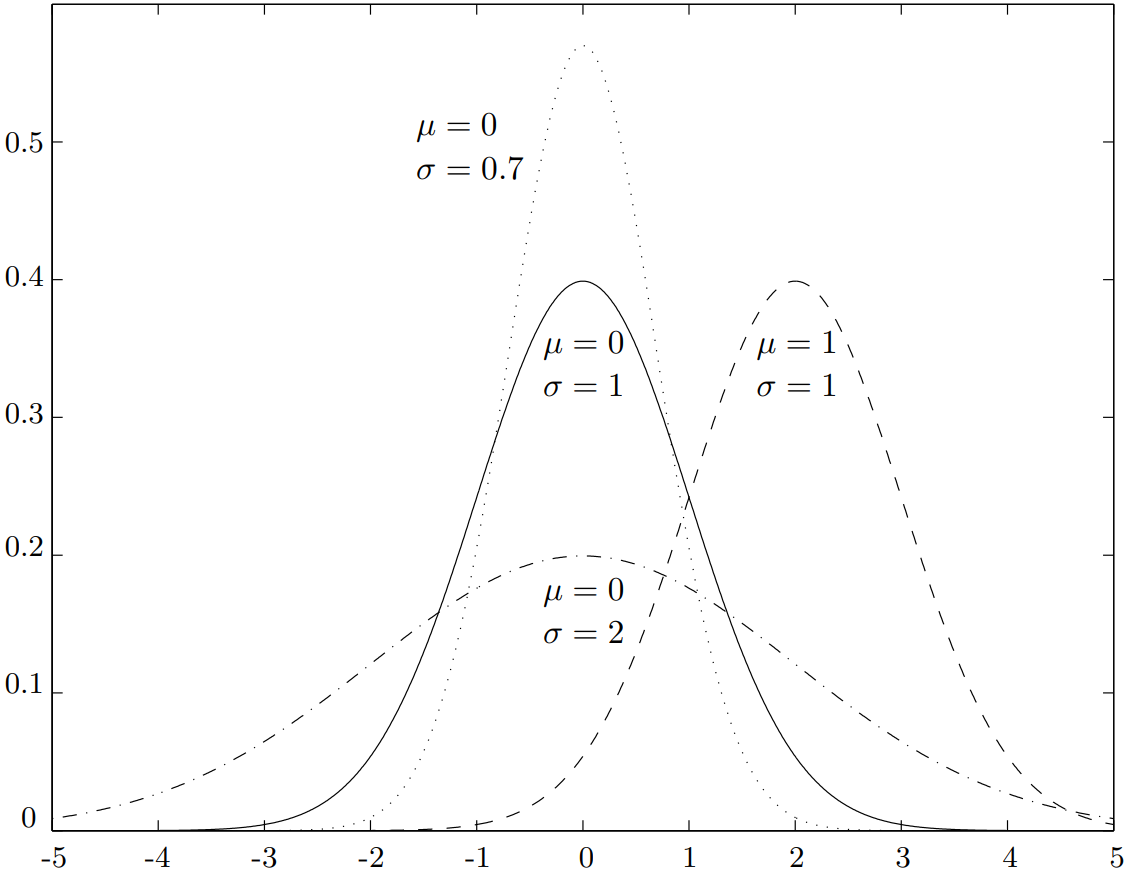
\includegraphics[width=.5\textwidth]{img/Fig4.6.png}
    \caption{\textit{Normal densities with different location and scale parameters.}}
\end{figure}

\subsubsection{Normal Distribution Functions and Variables}

\begin{formula}{}
    \begin{center}
        $\begin{aligned}
            \mu &= \textnormal{expectation, \textit{location} parameter}\\
            \sigma &= \textnormal{standard deviation, \textit{scale} parameter}\\
            f(x) &= \frac{1}{\sigma \sqrt[]{2 \pi}} \textnormal{exp}\left\{ \frac{-(x - \mu)^2}{2\sigma^2} \right\},\ \ \ \ -\infty < x < +\infty\\
            \expc{X} &= \mu\\
            \var{X} &= \sigma^2
        \end{aligned}$
    \end{center}
\end{formula}

\subsubsection{Standard Normal Distribution}

\begin{definition}{}
    Normal distribution with ``standard parameters'' $\mu = 0$ and $\sigma = 1$ is called \textbf{Standard Normal distribution}.
\end{definition}

\begin{formula}{NOTATION}
    \begin{center}
        $\begin{aligned}
            Z &= \textnormal{Standard Normal random variable}\\
            \phi(x) &= \frac{1}{\sqrt[]{2 \pi}} e^{-x^2/2},\textnormal{ Standard Normal pdf}\\
            \Phi(x) &= \int_{-\infty}^{x} \frac{1}{\sqrt[]{2 \pi}} e^{-z^2/2} dz, \textnormal{ Standard Normal cdf}
        \end{aligned}$
    \end{center}
\end{formula}

A Standard Normal variable, usually denoted by $Z$, can be obtained from a non-standard Normal($\mu, \sigma$) random variable $X$ by \textit{standardizing}, that is, subtracting the mean and dividing by the standard deviation,
\begin{equation}
    Z = \frac{X - \mu}{\sigma}
\end{equation}
\textit{Unstandardizing} $Z$, we can reconstruct the initial variable $X$,
\begin{equation}
    X = \mu + \sigma Z
\end{equation}
Using these transformations, any Normal random variable can be obtained from a Standard Normal variable $Z$; therefore, we need a table of Standard Normal Distribution only (Table A4 in book).

\begin{example}{: Computing non-standard Normal probabilities}
    Suppose that the average household income in some country is 900 coins, and the standard deviation is 200 coins. Assuming the Normal distribution of incomes, compute the proportion of ``the middle class'', whose income is between 600 and 1200 coins.

    \textbf{Solution:} Standardize and use Table A4. For a Normal($\mu = 900, \sigma = 200$) variable $X$,
    \begin{align*}
        \prob{600 < X < 1200} &= \prob{\frac{600 - \mu}{\sigma} < \frac{X - \mu}{\sigma} < \frac{1200 - \mu}{\sigma}}\\
        &= \prob{\frac{600 - 900}{200} < Z < \frac{1200-900}{200}} = \prob{-1.5 < Z < 1.5}\\
        &= \Phi(1.5) - \Phi(-1.5) = 0.9332 - 0.0668 = 0.8664
    \end{align*}
\end{example}

So far, we were computing probabilities of clearly defined events. These are direct problems. A number of applications require solution of an inverse problem, that is, finding a value of $x$ given the corresponding probability.

\begin{example_break}{: Inverse problem}
    The government of the country in Example 8 decides to issue food stamps to the poorest 3\% of households. Below what income will families receive food stamps?

    \textbf{Solution:} We need to find such income $x$ that $\prob{X < x} = 3\% = 0.03$. This is an equation that can be solved in terms of $x$. Again, we standardize first, then use the table:
    \begin{equation*}
        \prob{X < x} = \prob{Z < \frac{x - \mu}{\sigma}} = \Phi\left( \frac{x - \mu}{\sigma} \right) = 0.03,
    \end{equation*}
    from where
    \begin{equation*}
        x = \mu + \sigma\Phi^{-1}(0.03)
    \end{equation*}
    In Table A4, we have to find the probability, the table entry of 0.03. We see that $\Phi(-1.88) \approx 0.03$. Therefore, $\Phi^{-1}(0.03) = -1.88$, and
    \begin{equation*}
        x = \mu + \sigma(-1.88) = 900 + (200)(-1.88) = 524\ (coins)
    \end{equation*}
    is the answer. In the literature, the value $\Phi^{-1}(\alpha)$ is often denoted by $z_{1-\alpha}$.
\end{example_break}

As seen in this example, in order to solve an inverse problem, we use the table first, then unstandardize, as in (eq. 17), and find the required value of $x$.
